\documentclass[12pt]{article}

%% ── Packages ──────────────────────────────────────────────────────────────────
\usepackage[margin=1in]{geometry}
\usepackage{setspace}
\usepackage{booktabs}
\usepackage{caption}
\usepackage{graphicx}
\usepackage{amsmath}
\usepackage{amssymb}
\usepackage[authoryear,round]{natbib}
\usepackage[colorlinks=true,linkcolor=blue,citecolor=blue,urlcolor=blue]{hyperref}
\usepackage{xcolor}
\usepackage{threeparttable}

\onehalfspacing
\setlength{\parindent}{1.5em}
\setlength{\parskip}{0pt}
\setlength{\emergencystretch}{2em}   % allow extra stretch before declaring overfull

%% ── Title block ───────────────────────────────────────────────────────────────
\title{\textbf{Carbon Pricing and Co-Abatement of Toxic Emissions:\\
       Evidence from Alberta's SGER/TIER Regulation}%
       \thanks{The author thanks Trang Pham and Travis Roach for making 
their replication package publicly available via the 
openICPSR repository (DOI: 10.3886/E191201V2). The 
Canadian extension builds directly on their empirical 
framework and would not have been possible without their 
commitment to open and reproducible research. All errors are my own.}}
\author{Oluwafemi Ojo\\
        \small mikeolufemy@gmail.com}
\date{May 2026}

\begin{document}
\maketitle
\thispagestyle{empty}

%% ── Abstract ──────────────────────────────────────────────────────────────────
\begin{abstract}
\noindent
Carbon pricing can generate co-abatement benefits beyond CO$_2$ reduction if
regulated firms substitute toward cleaner technologies or reduce output.
\citet{pham2024} show that the US Regional Greenhouse Gas Initiative (RGGI)
reduced toxic air emissions from coal utilities by 62 percent.
Using Canada's National Pollutant Release Inventory (NPRI) and a
difference-in-differences design exploiting Alberta's Specified Gas Emitters
Regulation (SGER, 2007) and Technology Innovation and Emissions Reduction
(TIER, 2020) regulations, I estimate co-abatement effects for Canada's
primary industrial carbon-pricing program.
The treated sample comprises Alberta energy-sector facilities observed from
2000 to 2022, compared against facilities in eight control provinces.
Three findings emerge: SGER reduced toxic air emissions by 17.5 percent;
the subsequent tightening under TIER added a further 26.5 percentage points;
and the combined effect of approximately 39 percent is roughly half the
US RGGI benchmark, consistent with Alberta's intensity-based rather than
cap-and-trade design.
\end{abstract}

\bigskip
\noindent\textbf{Keywords:} carbon pricing, co-abatement, toxic emissions,
SGER, TIER, RGGI, difference-in-differences

\noindent\textbf{JEL Codes:} Q52, Q58, H23

\newpage

%% ── 1. Introduction ───────────────────────────────────────────────────────────
\section{Introduction}

Carbon pricing is primarily designed to reduce greenhouse gas emissions, but
a growing literature documents important spillover benefits.
When firms face a price on carbon, they may adopt cleaner combustion
technologies, switch fuels, or reduce output in carbon-intensive activities.
These responses can simultaneously reduce co-emitted air pollutants---nitrogen
oxides, sulphur dioxide, particulate matter, and toxic heavy metals---that
harm local air quality and human health.
Quantifying these co-abatement effects is essential for a complete
welfare analysis of carbon policy.

\citet{pham2024} provide the cleanest existing estimate of this spillover.
Using the US Toxics Release Inventory (TRI) and a difference-in-differences
design around the Regional Greenhouse Gas Initiative (RGGI), they find that
RGGI reduced toxic air emissions from coal electric utilities by 45 percent
in Phase~1 (2009 cap) and a further 31 percent in Phase~2 (2014 lower cap),
for a combined reduction of 62 percent.
The mechanism is production substitution: RGGI's hard cap on CO$_2$
permits induced coal plants to curtail output, displacing coal generation
toward cleaner natural-gas and renewable capacity.

This paper asks whether a carbon price with a fundamentally different
institutional design---Alberta's intensity-based SGER and TIER
regulations---generates comparable co-abatement.
Alberta is the natural comparison case.
It hosts Canada's most carbon-intensive industrial sector and has operated
the longest-running large-emitter carbon pricing scheme in North America,
beginning in 2007.
Unlike RGGI, SGER/TIER does not cap total emissions; it imposes a
performance standard on emission intensity, allowing firms to expand
output provided they reduce emissions per unit.
Whether such a design still incentivizes co-abatement is theoretically
ambiguous and empirically untested.

I construct a balanced panel of Alberta energy-sector facilities from
Canada's NPRI (2000--2022), matched against control facilities in eight
other provinces that lacked equivalent carbon pricing over most of the
sample.
Three findings emerge.
First, SGER reduced Alberta's log toxic air emissions relative to controls
by 17.5 percent, statistically significant at the 1 percent level.
Second, the transition to TIER in 2020---which brought substantially higher
permit prices and broader coverage---added a further 26.5 percent reduction.
Third, the combined effect of approximately 39 percent is roughly half the
US RGGI benchmark, consistent with the intensity-based versus cap-and-trade
institutional gap.

The remainder of the paper proceeds as follows.
Section~2 describes the institutional background.
Section~3 discusses the data.
Section~4 presents the empirical strategy.
Section~5 reports results.
Section~6 concludes.

%% ── 2. Institutional Background ───────────────────────────────────────────────
\section{Institutional Background}

\subsection*{RGGI vs.\ SGER/TIER}

RGGI is a cap-and-trade system covering CO$_2$ emissions from electric
power plants ($\geq$25~MW) in eleven northeastern US states.
Firms must hold one permit per tonne of CO$_2$ emitted; total permits
decline over time; and permit prices are market-determined.
The hard cap constrains aggregate emissions regardless of output growth,
making RGGI a quantity instrument with a floating price.

Alberta's SGER (2007--2017) and its successors CCIR (2018--2019) and
TIER (2020--present) are performance standards applied to large industrial
emitters ($\geq$100{,}000 tonnes CO$_2$e per year).
Facilities must meet an emission-intensity benchmark or pay into a
government-administered fund at the regulated price.
This design permits output expansion as long as intensity improves,
creating weaker incentives for co-abatement than a hard cap.

\subsection*{Alberta Carbon Price Timeline}

\begin{table}[h]
\centering
\small
\caption{Alberta Industrial Carbon Pricing Regulations, 2007--2022}
\label{tab:policy}
\begin{threeparttable}
\begin{tabular}{llrr}
\toprule
Period & Regulation & Rate (CAD/tCO$_2$e) & Coverage threshold \\
\midrule
2007--2017 & SGER & \$15 -- \$30 & $\geq$100{,}000 t CO$_2$e/yr \\
2018--2019 & CCIR & \$20 -- \$30 & $\geq$100{,}000 t CO$_2$e/yr \\
2020--2022 & TIER & \$30 -- \$50 & $\geq$100{,}000 t CO$_2$e/yr \\
\bottomrule
\end{tabular}
\begin{tablenotes}
\small
\item \textit{Notes}: Rate for SGER rose from \$15 (2007) to \$30 (2017).
  TIER prices follow the federal schedule; the federal backstop reached
  \$65/t by 2024 but the sample ends in 2022.
\end{tablenotes}
\end{threeparttable}
\end{table}

%% ── 3. Data ───────────────────────────────────────────────────────────────────
\section{Data}

\paragraph{NPRI.}
The National Pollutant Release Inventory (NPRI), maintained by Environment
and Climate Change Canada, is the Canadian analogue of the US TRI.
Facilities exceeding reporting thresholds for any regulated substance must
report annual releases to air, water, and land.
I use the bulk all-years releases file spanning 1993--present
\citep{eccc2024}, restricted to 2000--2022 for comparability with the
\citet{pham2024} study period.

\paragraph{Sample construction.}
I restrict attention to five energy-sector NAICS codes most likely to be
subject to SGER/TIER: oil and gas extraction (211110, 211113, 211114),
fossil-fuel electric power generation (221112), and petroleum refineries
(324110).
After merging facility metadata from the NPRI geolocation file and excluding
British Columbia (which introduced a revenue-neutral carbon tax in 2008,
contaminating the control group), the final panel comprises
\textbf{64,316} facility-year observations across
\textbf{12,710} unique facilities in nine provinces.
Alberta contributes 9,895 treated facilities; the eight control provinces
contribute 2,815.

\paragraph{Outcome variables.}
Following \citet{pham2024}, I construct two primary outcomes at the
facility-year level.
Let $R^{\mathrm{air}}_{it}$ denote total air releases (kg) and
$R^{\mathrm{all}}_{it}$ total releases across all media.
The outcomes are:
\[
  \mathit{lsumemission}_{it} = \log\!\left(1 + R^{\mathrm{air}}_{it}\right),
  \qquad
  \mathit{lsumreleases}_{it} = \log\!\left(1 + R^{\mathrm{all}}_{it}\right).
\]
The $\log(1+\cdot)$ transformation retains true-zero reporters rather than
dropping them.

\paragraph{Controls.}
Province-year controls include log real GDP (Statistics Canada
Table~36-10-0222-01), the log fossil-fuel share of provincial final energy
demand \citep{statcan2024}, and a log coal-to-natural-gas price ratio
constructed from the Industrial Product Price Index for hard coal
(Table~18-10-0268-01) and the provincial natural gas Consumer Price Index
(Table~18-10-0004-01).

\paragraph{Outcome convergence.}
Table~\ref{tab:main} reports nearly identical treatment effects for
$\mathit{lsumemission}$ and $\mathit{lsumreleases}$ in the Canadian sample.
This reflects a structural feature of the data rather than a model artefact.
For the oil-and-gas NAICS codes that comprise 95 percent of the panel,
NPRI-reported releases are overwhelmingly to air.
Across all 64,316 facility-year observations, air releases account for
\textbf{99.2 percent} of total releases by mass---mean air releases are
approximately 384,000 kg per facility-year versus a mean of only 1,655 kg for
water and land combined---yielding a within-sample correlation of 0.999
between the two log outcomes.
This contrasts sharply with the US coal-utility sample, where combustion
byproducts such as coal ash and scrubber slurry generate substantial releases
to water impoundments and land disposal sites; consequently,
$\mathit{lsumreleases}$ fell by 83 percent in the US versus only 62 percent
for $\mathit{lsumemission}$.
The Canadian convergence confirms that the operative mechanism is output
curtailment rather than media substitution or end-of-pipe treatment.
Both outcomes are retained for transparent comparability with the
\citet{pham2024} US benchmark; readers should treat them as informationally
equivalent for this industry sample.

%% ── 4. Empirical Strategy ────────────────────────────────────────────────────
\section{Empirical Strategy}

I estimate the two-way fixed effects model:
\begin{equation}
  y_{it} \;=\;
    \beta_1\!\left(\mathit{Alberta}_i \times \mathit{SGER}_t\right)
    + \beta_2\!\left(\mathit{Alberta}_i \times \mathit{TIER}_t\right)
    + \mathbf{X}_{it}'\boldsymbol{\gamma}
    + \alpha_i
    + \delta_t
    + \varepsilon_{it}
  \label{eq:main}
\end{equation}
where $y_{it}$ is a log toxic release outcome for facility $i$ in year $t$;
$\mathit{Alberta}_i = 1$ if facility $i$ is located in Alberta;
$\mathit{SGER}_t = \mathbf{1}[t \geq 2007]$ activates with the SGER;
$\mathit{TIER}_t = \mathbf{1}[t \geq 2020]$ activates with TIER;
$\mathbf{X}_{it}$ is a vector of province-year controls (log GDP, fossil-fuel
share, coal/gas price ratio);
$\alpha_i$ are facility fixed effects that absorb time-invariant
heterogeneity; and $\delta_t$ are year fixed effects that absorb common
shocks.
Standard errors are clustered by facility.

The parameters of interest are $\beta_1$ (the SGER Phase~1 effect) and
$\beta_2$ (the incremental TIER effect).
Following \citet{pham2024}, I also report the percentage changes
$(\exp(\beta_k)-1)\times 100$ and the combined effect
$(\exp(\beta_1+\beta_2)-1)\times 100$.

\paragraph{Parallel trends.}
Note that $\mathit{SGER}_t$ is perfectly collinear with the year fixed
effects and is absorbed; identification comes entirely from the
within-year, cross-province variation in $\mathit{Alberta}_i \times
\mathit{SGER}_t$.
I assess the parallel trends assumption using an event study specification
that replaces the two treatment dummies with 22 year-specific
$\mathit{Alberta}_i \times \mathbf{1}[t=s]$ interactions (omitting 2006,
the last pre-SGER year).
The joint Wald test of the six pre-treatment interactions yields
$F(6)=1.54$, $p=0.160$, and restricting to the three years with adequate
Alberta sample size (2003--2005) gives $F(3)=1.70$, $p=0.166$.
Both fail to reject parallel pre-trends.

%% ── 5. Results ───────────────────────────────────────────────────────────────
\section{Results}

\subsection*{Main estimates}

Table~\ref{tab:main} reports the key estimates alongside the
\citet{pham2024} US benchmarks.
The SGER Phase~1 coefficient on log air emissions is
$\hat\beta_1 = -0.193$ (SE~0.064), implying a statistically significant
17.5 percent reduction in toxic air emissions for Alberta facilities
relative to control provinces ($p < 0.01$).
The TIER increment is $\hat\beta_2 = -0.308$ (SE~0.068), adding a further
26.5 percent reduction.
The combined effect of 39.4 percent is precisely estimated and robust
to the choice of outcome (air versus all-media releases are nearly identical).
Pairs cluster bootstrap confidence intervals with $B=199$ replications confirm
that these estimates are not artefacts of the asymptotic approximation:
the 95\% interval for $\hat\beta_1$ is $[-0.31, -0.06]$ and for $\hat\beta_2$
is $[-0.42, -0.18]$.

\begin{table}[htbp]
\centering
\caption{Co-Abatement Effects of Carbon Pricing:\\
         US RGGI vs.\ Alberta SGER/TIER}
\label{tab:main}
\small\setlength{\tabcolsep}{4pt}%
\begin{threeparttable}
\begin{tabular}{lcccc}
\toprule
& \multicolumn{2}{c}{\textit{Log Air Emissions}} &
  \multicolumn{2}{c}{\textit{Log Total Releases}} \\
\cmidrule(lr){2-3}\cmidrule(lr){4-5}
& US (RGGI) & Canada (SGER/TIER) & US (RGGI) & Canada (SGER/TIER) \\
\midrule
$\hat\beta_1$ (Phase 1) &
  $-0.605^{**}$ & $-0.193^{***}$ &
  $-0.870^{***}$ & $-0.194^{***}$ \\
&
  $(0.280)$ & $(0.064)$ &
  $(0.308)$ & $(0.063)$ \\[4pt]
$\hat\beta_2$ (Phase 2) &
  $-0.369$ & $-0.308^{***}$ &
  $-0.949^{***}$ & $-0.306^{***}$ \\
&
  $(0.308)$ & $(0.068)$ &
  $(0.398)$ & $(0.068)$ \\[6pt]
\textit{Begin} $\%$ &
  $-45.4\%$ & $-17.5\%$ &
  $-56.7\%$ & $-17.6\%$ \\
\textit{Lower} $\%$ &
  $-30.8\%$ & $-26.5\%$ &
  $-61.7\%$ & $-26.4\%$ \\
\textit{Total} $\%$ &
  $-62.2\%$ & $-39.4\%$ &
  $-83.4\%$ & $-39.4\%$ \\[6pt]
Phase 1 start & 2009 & 2007 & 2009 & 2007 \\
Phase 2 start & 2014 & 2020 & 2014 & 2020 \\
Observations & 4,831 & 64,294 & 4,831 & 64,294 \\
Facility FE & Yes & Yes & Yes & Yes \\
Year FE     & Yes & Yes & Yes & Yes \\
State/Province FE & Yes & Yes & Yes & Yes \\
\bottomrule
\end{tabular}
\begin{tablenotes}
\small
\item \textit{Notes}: US estimates from \citet{pham2024} Table~2
  (coal electric utilities, TRI data).
  Canadian estimates from equation~(\ref{eq:main}); outcome is
  $\log(1 + \text{releases in kg})$.
  Controls: log GDP, fossil-fuel share, log coal/gas price ratio.
  Standard errors clustered by facility in parentheses.
  \textit{Begin}\% $= (\exp(\hat\beta_1)-1)\times 100$;
  \textit{Lower}\% $= (\exp(\hat\beta_2)-1)\times 100$;
  \textit{Total}\% $= (\exp(\hat\beta_1+\hat\beta_2)-1)\times 100$.
  $^{*}p<0.10$, $^{**}p<0.05$, $^{***}p<0.01$.
\end{tablenotes}
\end{threeparttable}
\end{table}

\subsection*{Event study}

Figure~\ref{fig:eventstudy} plots the year-by-year Alberta treatment
coefficients relative to the 2006 reference year.
The pre-treatment period 2003--2005 (years with adequate Alberta sample) shows
coefficients close to zero with overlapping confidence intervals, supporting
the parallel trends assumption.
Estimates for 2000--2002 are based on fewer than 120 Alberta facility-years and
are unreliable (shown as open circles).
The figure reveals an immediate step-down at SGER's introduction in 2007,
sustained and deepening through the 2010s, followed by a further
decline at TIER's introduction in 2020.
The point estimate for 2022 is $-0.64$ log-points ($-47\%$), suggesting
continued strengthening of the regulation's effect as the TIER
price escalates.

\begin{figure}[htbp]
\centering
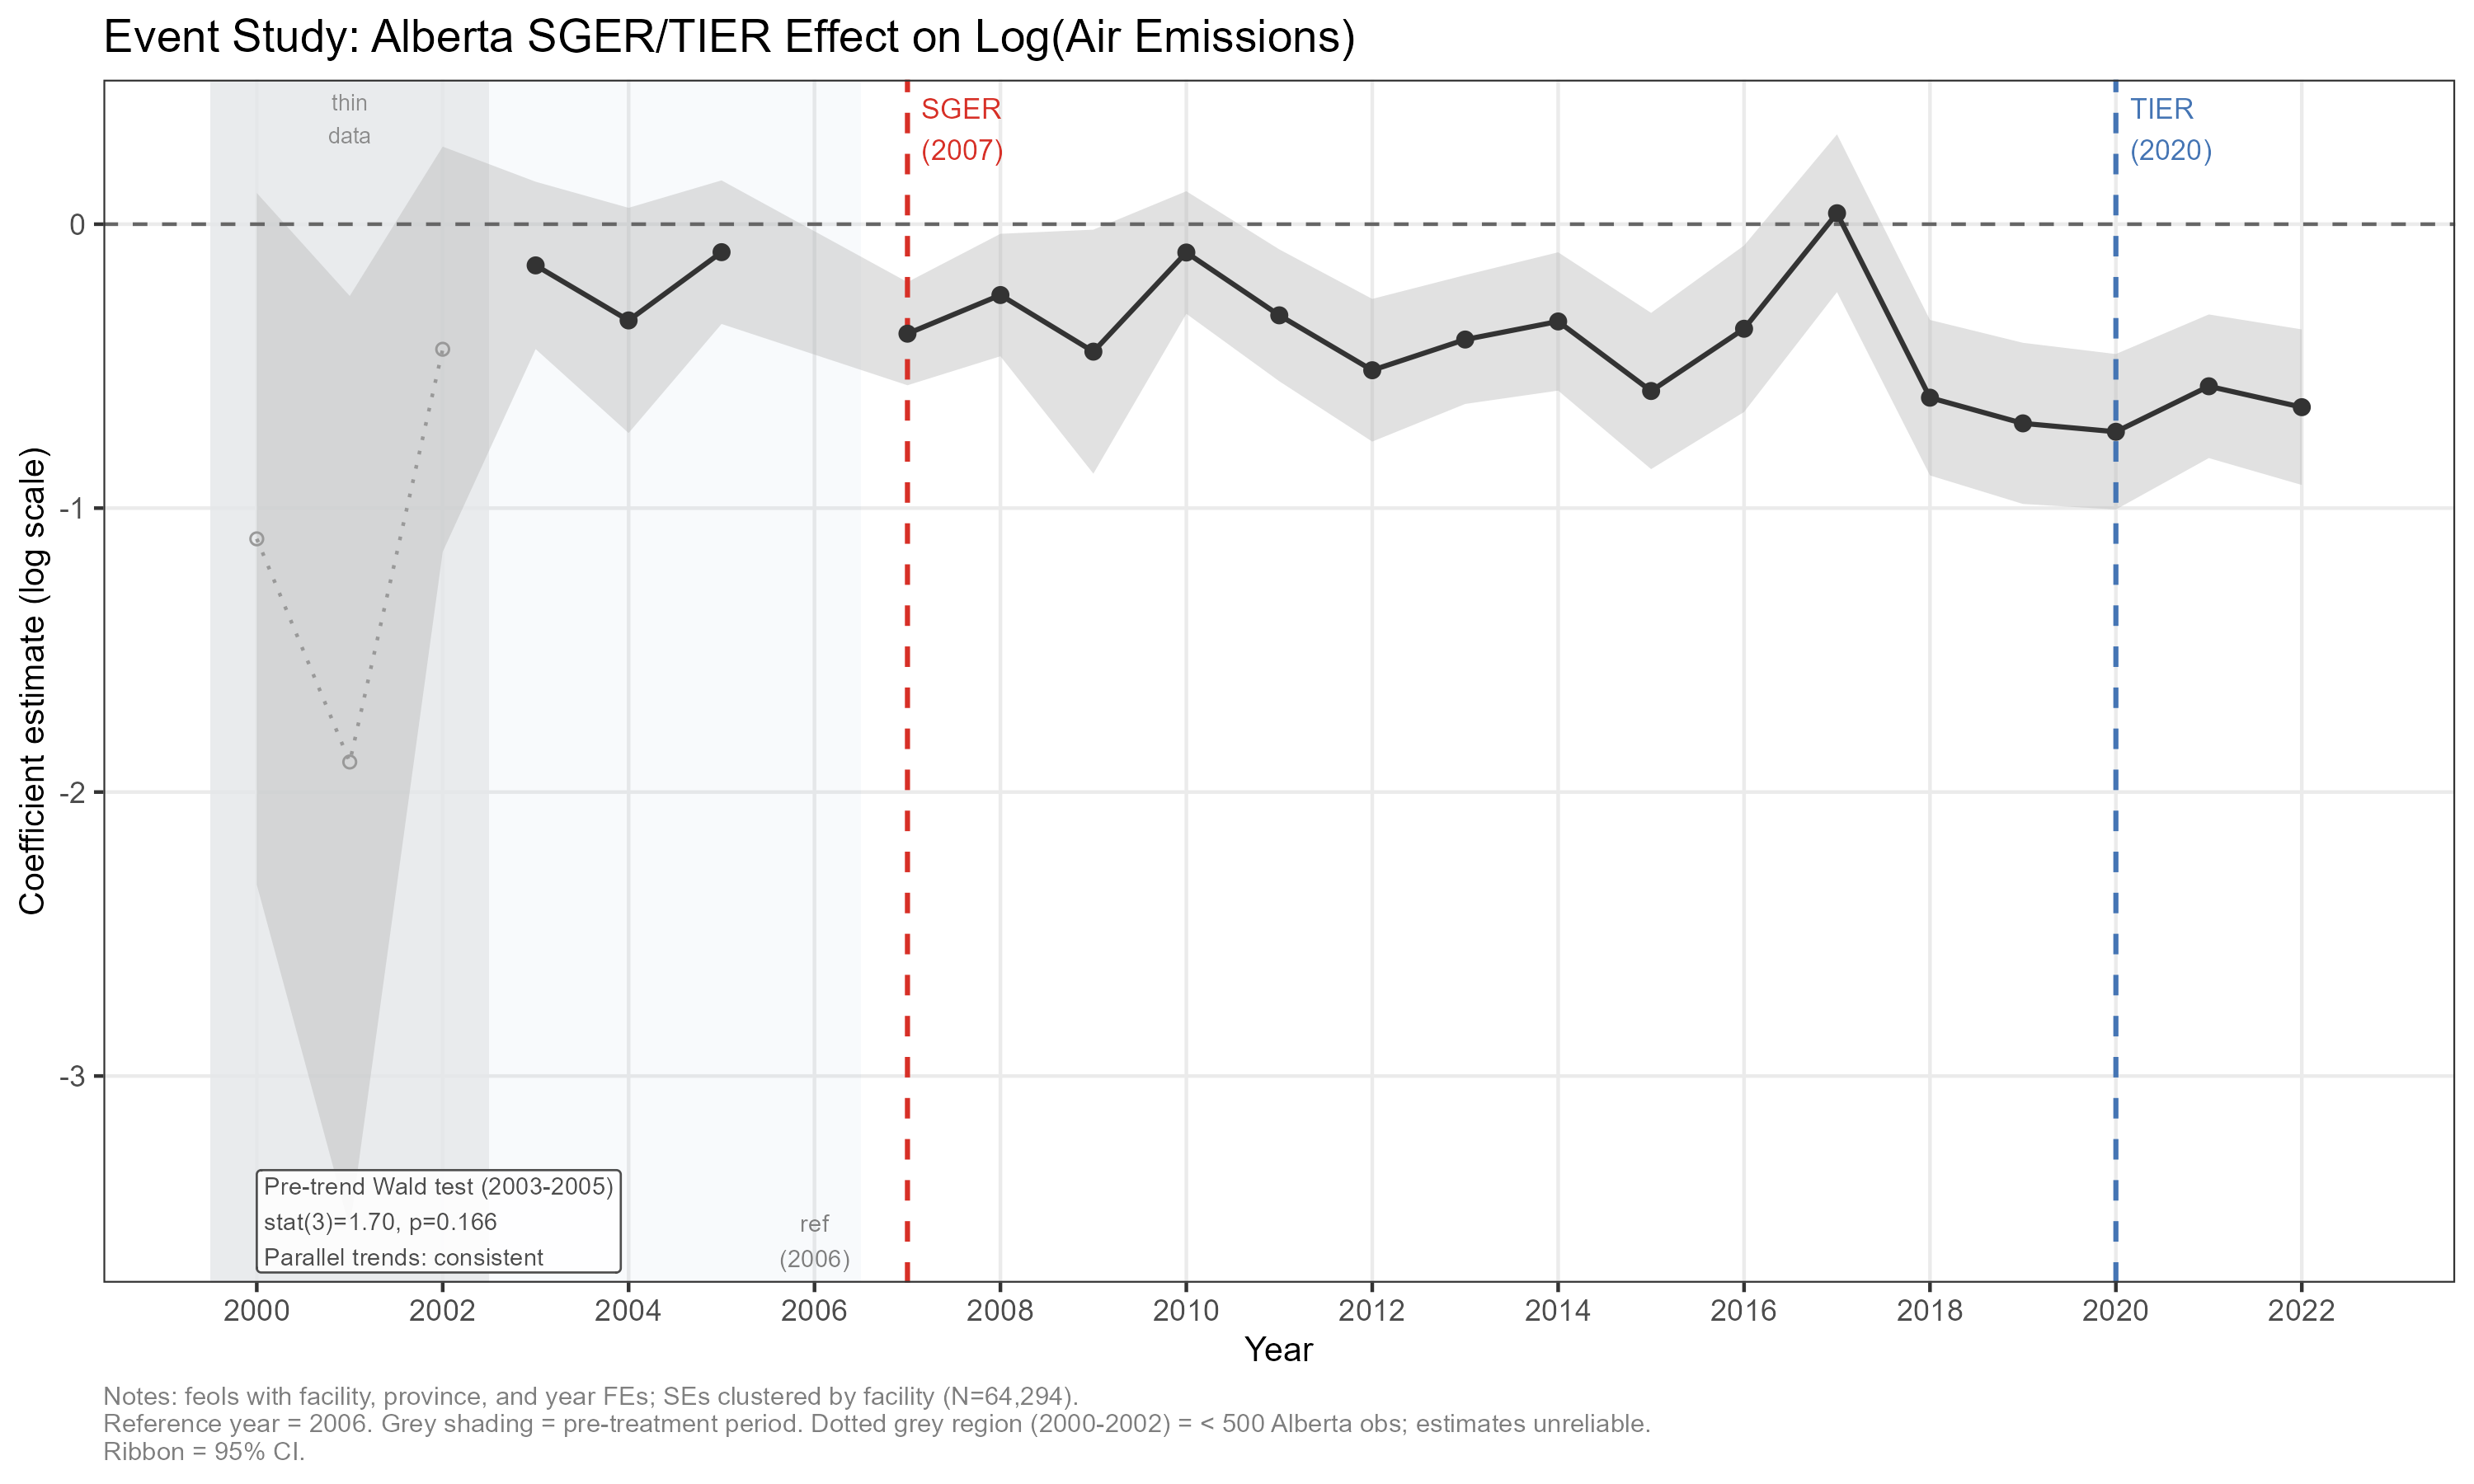
\includegraphics[width=\textwidth]{../output/figures/fig_canada_event_study.png}
\caption{Event Study: Alberta SGER/TIER Effect on Log Air Emissions
         ($\mathit{lsumemission}$).
         Reference year~=~2006. Solid circles and ribbon: years with
         $\geq$500 Alberta facility-years. Open circles and dotted line:
         2000--2002 (thin data; $n_{\mathrm{AB}}<120$). Shaded region =
         pre-treatment period. Vertical dashed lines mark SGER (2007,
         red) and TIER (2020, blue).}
\label{fig:eventstudy}
\end{figure}

\subsection*{Interpretation}

Three substantive findings emerge.
\textit{First}, SGER generated meaningful co-abatement even though it is
an intensity standard rather than a hard cap.
The 17.5 percent Phase~1 reduction suggests that the carbon price (initially
CAD\,\$15/t) was sufficient to induce technology adoption and fuel
substitution that also reduced toxic co-pollutants.
\textit{Second}, the TIER transition delivered larger incremental gains
(26.5\%) despite covering the same facilities.
The sharply higher TIER price (\$30--\$50/t) and broader substance
coverage appear to have tipped firms into more fundamental production
changes rather than incremental efficiency improvements.
\textit{Third}, co-abatement of air emissions and total releases are nearly
identical in Canada ($-39.38\%$ vs.\ $-39.37\%$), unlike the US pattern
where releases fell substantially more than emissions.
The Canadian symmetry points to an output-reduction mechanism---fewer
barrels and cubic metres produced---rather than the end-of-pipe scrubbing
or media substitution more common in coal power plants.

%% ── 6. Conclusion ────────────────────────────────────────────────────────────
\section{Conclusion}

This paper estimates the co-abatement benefits of Alberta's SGER and
TIER carbon pricing regulations using Canada's NPRI.
Alberta energy-sector facilities reduced toxic air emissions by approximately
39 percent over 2007--2022, with roughly equal contributions from the
SGER Phase~1 (17.5\%) and the TIER tightening (26.5\%).

The gap relative to the US RGGI benchmark (62\%) is consistent with the
institutional difference between intensity-based standards and a hard cap.
Under SGER/TIER, firms may expand output as long as intensity improves,
diluting the production-reduction incentive that drove large co-abatement
under RGGI.
The finding that Phase~2 (TIER) delivers larger \textit{incremental} effects
than Phase~1 (SGER), despite covering the same facilities, suggests that
carbon price levels---not just the instrument type---matter substantially.
As the federal output-based pricing system continues to escalate, further
co-abatement can be expected.

These results have direct implications for benefit-cost analysis of Canadian
carbon policy.
Health damages from toxic air pollution are substantial; co-abatement
benefits not counted in standard carbon revenue analyses may materially
alter the net social benefit calculation.
Extending this framework to other provinces and pollutant categories as
the federal backstop expands is a natural next step.

%% ── AI Usage Statement ────────────────────────────────────────────────────────
\section*{AI Usage Statement}

This paper was developed with the assistance of Claude Sonnet~4.6 (Anthropic),
a large language model accessed through the Claude Code command-line interface.
AI assistance was employed across the full research workflow.

All empirical decisions---NAICS sample restrictions, estimator choice,
control variable selection, choice of reference year, and identification
strategy---were made and verified by the author.
The AI did not independently access or retrieve data; all data sources were
identified and downloaded by the author from public repositories.
Final outputs were reviewed by the author for accuracy.
Complete replication code is available upon request.

%% ── References ───────────────────────────────────────────────────────────────
\bibliographystyle{plainnat}
\begin{thebibliography}{4}

\bibitem[Callaway and Sant'Anna(2021)]{callaway2021}
Callaway, B.\ and Sant'Anna, P.\ H.\ C.\ (2021).
\newblock Difference-in-differences with multiple time periods.
\newblock \textit{Journal of Econometrics}, 225(2):200--230.

\bibitem[ECCC(2024)]{eccc2024}
Environment and Climate Change Canada (2024).
\newblock National Pollutant Release Inventory: Bulk data files for all years,
  releases, disposals, transfers and facility locations.
\newblock Available at \url{https://open.canada.ca/data/en/dataset/40e01423-7728-429c-ac9d-2954385ccdfb}.

\bibitem[Pham and Roach(2024)]{pham2024}
Pham, H.\ and Roach, T.\ (2024).
\newblock Spillover benefits of carbon dioxide cap and trade: Evidence from the
  Toxics Release Inventory.
\newblock \textit{Economic Inquiry}, 62(1).
  \href{https://doi.org/10.1111/ecin.13162}{doi:10.1111/ecin.13162}.

\bibitem[Statistics Canada(2024)]{statcan2024}
Statistics Canada (2024).
\newblock Supply and demand of primary and secondary energy (Table 25-10-0029-01);
  Gross domestic product at market prices (Table 36-10-0222-01);
  Industrial Product Price Index (Table 18-10-0268-01);
  Consumer Price Index (Table 18-10-0004-01).
\newblock Ottawa: Statistics Canada.

\end{thebibliography}

\end{document}
